\documentclass[a4paper,addpoints,12pt]{exam}

\usepackage{dlds}






\begin{document}





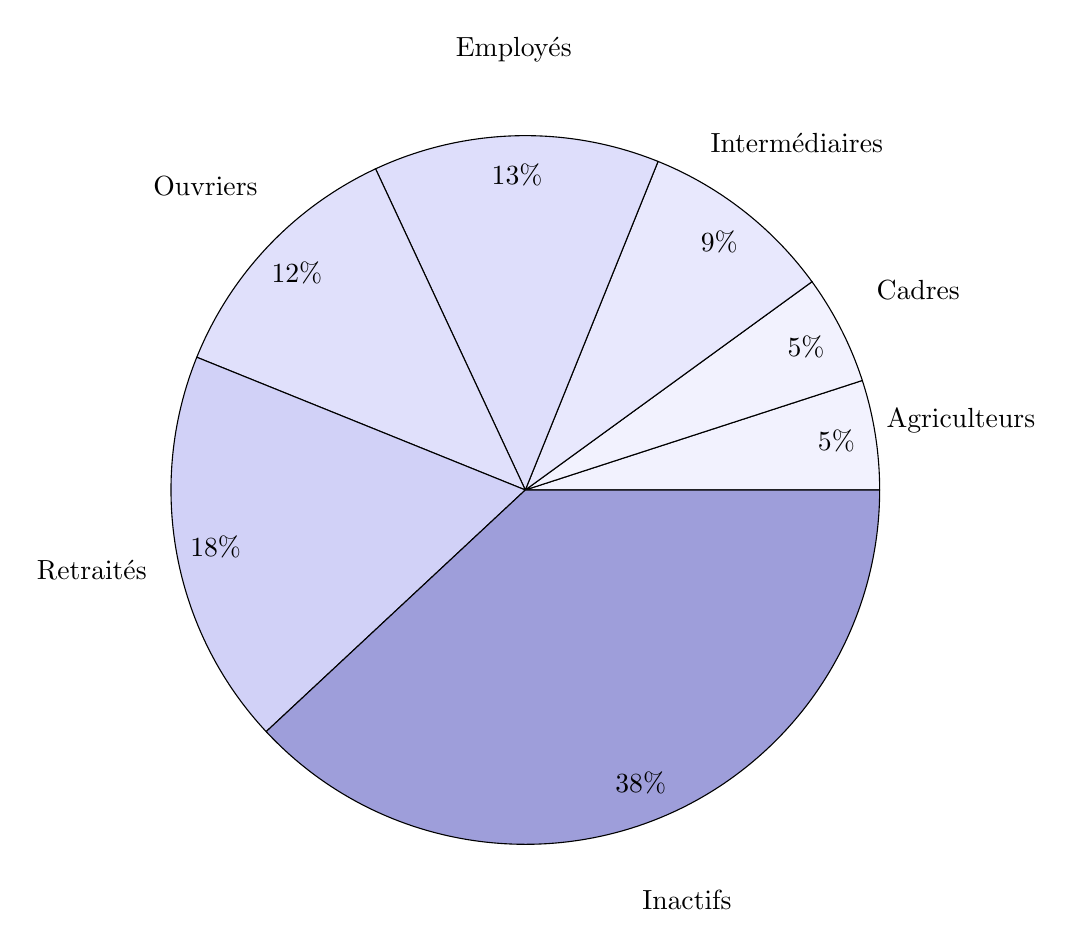
\begin{tikzpicture}
\foreach \a/\b/\p/\c in
{
0/18/5/Agriculteurs, 18/36/5/Cadres, 36/68/9/Intermédiaires, 68/115/13/Employés,  115/158/12/Ouvriers, 158/223/18/Retraités, 223/360/38/Inactifs
}
{
\draw[fill=black!\p!blue!\p]
(0,0) -- (\a:4.5) arc (\a:\b:4.5) -- cycle;
\draw ({(\a+\b)/2}:4) node {\p\%};
\draw ({(\a+\b)/2}:5.6) node {\c};
}
\end{tikzpicture}

\end{document}